\documentclass[11pt, oneside]{article}   	% use "amsart" instead of "article" for AMSLaTeX format
\usepackage{geometry}                		% See geometry.pdf to learn the layout options. There are lots.
\geometry{letterpaper}                   		% ... or a4paper or a5paper or ... 
%\geometry{landscape}                		% Activate for rotated page geometry
%\usepackage[parfill]{parskip}    		% Activate to begin paragraphs with an empty line\usepackage{graphicx}				% Use pdf, png, jpg, or eps§ with pdflatex; use eps in DVI mode
								% TeX will automatically convert eps --> pdf in pdflatex
								
%\usepackage{{Gratzer-Color-Scheme}	% Active to color theorems red and lemmas blue
	
\usepackage{amssymb}
\usepackage{amsmath}
\usepackage{amsthm}
\usepackage{tikz}

\usepackage{enumitem}
\usepackage{xcolor}

\usepackage{hyperref}

\newtheorem{theorem}{Theorem}[section]
\newtheorem{corollary}{Corollary}[section]
\newtheorem{lemma}{Lemma}[section]
\newtheorem{proposition}{Proposition}[section]

\theoremstyle{definition}
\newtheorem{definition}{Definition}[section]
\newtheorem{example}{Example}[section]

\theoremstyle{remark}
\newtheorem*{remark}{Remark}

%SetFonts

%SetFontsfiley


\title{Understanding the Poisson Process}
\author{James A. Rose}
%\date{}							% Activate to display a given date or no date

\begin{document}
\maketitle

\tableofcontents

\newpage
\section{History of the Poisson Process} \label{history}
To build an understanding of the Poisson process, it is important to look at how it originated and how we arrived at the definition of the Poisson process that we will use throughout the paper. I will refer back to the origins discussed here because they provide a powerful intuition about how the process works and where we can apply it.

History about Siméon Poisson and ideas for the following derivation can be found in \cite{poisson2026}.

The origins date back to 1837, when Siméon Denis Poisson released his paper on the Probability of Judgments in Criminal and Civil Matters. The Poisson distribution is derived as a limit of the Binomial distribution.

\vspace{5mm}

Suppose we perform an experiment with $n$ independent trials, each with a small probability, $p$, of success. Let $X_n \sim \textit{Binomial}(n,p)$, so $X_n$ denotes the number of successful trials. Then, for a fixed $k$, the pmf is $$\mathbb{P}(X_n=k)=\binom{n}{k}p^k(1-p)^{n-k}.$$

As we take $n\to\infty$ and $p\to0$, we should converge to the Poisson distribution. 
Fix $\lambda=np$. Take $n\to\infty$ ($p\to0$ because $\lambda$ is fixed), then:

\begin{enumerate}[label=(\roman*)] 
  \item \begin{align*}
      \binom{n}{k} p^k &= \frac{n(n-1)...(n-k+1)}{k!}\cdot \left(\frac{\lambda}{n}\right)^k = \frac{n(n-1)...(n-k+1)}{n^k}\cdot \frac{\lambda^k}{k!} \\
		       &= \frac{n}{n}\cdot\frac{n-1}{n}...\frac{n-k+1}{n}\cdot \frac{\lambda^k}{k!} = 1\cdot\left( 1-\frac{1}{n}\right)...\left( 1-\frac{k-1}{n}\right)\cdot \frac{\lambda^k}{k!} \to \frac{\lambda^k}{k!},
    \end{align*}
  \item $$\left(1-\frac{\lambda}{n}\right)^{n-k}=\left(1-\frac{\lambda}{n}\right)^n\cdot\left(1-\frac{\lambda}{n}\right)^{-k} \to e^{-\lambda}\cdot 1 = e^{-\lambda}.$$
\end{enumerate}

Therefore, we can determine what the Binomial distribution converges to:
$$\mathbb{P}(X_n=k)\to\frac{\lambda^k e^{-\lambda}}{k!} \hspace{5mm}\text{ as } n\to\infty$$

Hence, we have that the limit of a Binomially distributed random variable is Poisson distributed.

\vspace{5mm}

Early in the 20th century, Rutherford observed particles in radioactive decay. He noticed the following:

\begin{enumerate}[label=(\roman*)]
  \item the decay events occurred at random times,
  \item the number of decays in a fixed time interval followed a pattern (the Poisson distribution),
  \item the waiting times were exponentially distributed.
\end{enumerate}
He was observing the Poisson process, but at this point, there was no formal definition for it.

William Feller later gave a rigorous definition of the process \cite{feller1971}, and concluded a Poisson process, $N$, had these properties:
\begin{enumerate}[label=(\roman*)]
  \item independent increments (over disjoint intervals), i.e. for any $0\leq t_0 < ... < t_k$, the random variables, $N(t_1)-N(t_0),...,N(t_n)-N(t_{n-1})$, are independent,
  \item stationary increments, i.e. for any $0\leq t_1<t_2$, and $s>0$, $N(t_2+s)-N(t_1+s)$ has the same distribution as $N(t_2)-N(t_1)$,
  \item the probability of more than one event in a small time interval is negligible.
\end{enumerate}

And finally, in the mid-20th century, the following 3 definitions became standard for a Poisson process; these come from \cite{mit2011} and \cite{probability2-2024}.

\begin{definition} \label{def1}
  Let $(N(t))_{t\geq0}$ be a stochastic process, then $(N(t))_{t\geq0}$, sometimes just written as $N$, is a Poisson process with rate $\lambda$ if
  \begin{enumerate}[label=(\roman*)]
    \item $N(0)=0$, N is integer-valued and right-continuous,
    \item N has independent increments,
    \item for any $t\geq0$, as $h\searrow 0$, 
      $$\mathbb{P}\left(N(t+h)-N(t)=n\right) = \begin{cases} 1-\lambda h+o(h) &n=0 \\ \lambda h + o(h) &n=1 \\ o(h) &n\geq2. \end{cases}$$ 
      This implies $N$ has stationary increments.
  \end{enumerate}
\end{definition}

\begin{definition} Let $N$ be a stochastic process, then $N$ is a Poisson process with rate $\lambda$ if conditions $(i)$ and $(ii)$ from above are satisfied and
  \begin{enumerate}[label=(\roman*)]
    \setcounter{enumi}{2}
    \item for any $s,t\geq0$, $$N(t+s)-N(s) \sim \textit{Poisson}(\lambda t)$$
  \end{enumerate}
\end{definition}

\begin{definition} \label{def3}
  Let $(X_i)_{i\geq0}$ be a sequence of random variables such that \\$X_i\sim \textit{Exponential}(\lambda)$ and $S_n=\sum_{i=0}^n{X_i}$. Then $$N(t):=max\{n:S_n\leq t\}$$ is a \textit{Poisson process} with rate $\lambda$.
\end{definition}

Let's relate the derivation of the Poisson by the convergence of the Binomial distribution to the definition of the Poisson process, to build an intuition as to why the number of random events over time follows a Poisson distribution. 

Consider particle decay over a time interval $[0,t]$. Divide $[0,t]$ into $n$ time intervals $h=\frac{t}{n}$, such that $h$ is small. In each time interval, suppose there is an 'attempt' for a particle to decay, or several decays with negligible probability, then the probability of a decay in each interval is approximately \textit{Bernoulli}$(\lambda h)$. Then the total decays in the interval $[0,t]$ is approximately \textit{Binomial}$(n, \lambda h)$ if the decay events are independent for disjoint time intervals.


Take $n \to \infty$, 
$$\textit{Binomial}\left(n, \lambda h\right) \to \textit{Poisson}(\lambda t),$$
then we can see how William Feller's definition gives the Poisson process.

\vspace{5mm}

From William Feller's definition, we might guess that the Poisson process is distributed \textit{Uniformly}. The definition describes the Poisson process as the number of events that occur randomly in a time interval without pattern (independence) and with a constant rate. This guess turns out to be true; the property is called the order statistic property, and we will prove it later.
We will also see that the time of the next event is \textit{independent of the past}, which is characterised by the Exponential distribution of the waiting time between two events as in Definition \ref{def3}.

We would like to generalise this process, so before moving on to the next section, where we define the Poisson point process, let's define a non-homogeneous Poisson process. In the non-homogeneous case, the rate is not constant and is instead given by a function, $\mu$.
\begin{definition}
  Let $N$ be a stochastic process with a rate given by a function, $\mu$, and if $N$ satisfies properties $(i)$ and $(ii)$ from Definition \ref{def1}, and
  $$N(t) \sim \textit{Poisson}(\mu(t)),$$
  then $N$ is a \textit{non-homogeneous Poisson process}.
\end{definition}

The next section will build a definition for the Poisson point process.




\newpage
\section{Definition and Overview of the Poisson Point Process} \label{overview}
In this section, we will derive a definition for the Poisson point process, motivated by the Poisson process over time covered in the previous section. We will then explore some applications with examples. Definitions in this section come from \cite{resnick2005}.

\vspace{5mm}

First, we define a point process. Suppose $E$ is a subset of the Euclidean space $\mathbb{R}^n$ for some $n\geq 1$. Consider the Euclidean space $[0,\infty)$ for the process over time. We want to randomly distribute points in $E$ and define a function that counts points in a set. 

\begin{definition}[Point process] \label{pointprocess}
  Let $\{X_n\}_{n\geq 0}$ be a random sequence from the state space $E$ and $A$ be a bounded set. We define the function $N$ by
  $$ N(A):=\sum_{n}{\delta_{X_n} (A)} $$ 
  where $\delta_{x_i}$, the Dirac measure at $x_i$, is defined by
  $$\delta_{x_i}(A) = \begin{cases} 1 &\text{if } x_i \in A \\ 0 &\text{if } x_i \notin A \end{cases}.$$ 
  We call $N$ a \textit{point process}.
\end{definition}

Then $\{X_n\}$ represents the random points in $E$, and $N$ is a counting measure for the total number of points that fall in $A$.

\begin{figure}
  \centering
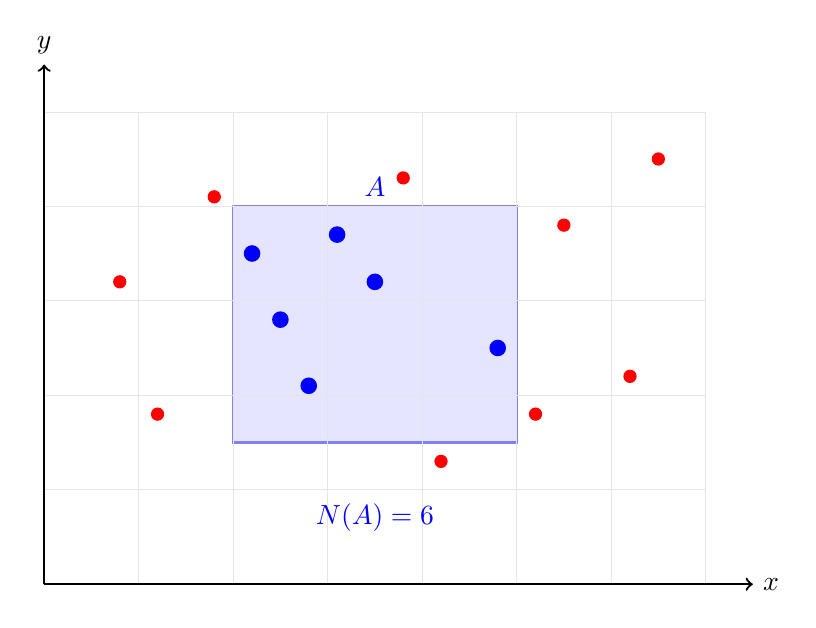
\begin{tikzpicture}[scale=1.2]
\filldraw[fill=blue!10, draw=blue!50, thick] (2,1.5) rectangle (5,4);
\node[blue] at (3.5,4.2) {$A$};

\draw[gray!20, very thin] (0,0) grid (7,5);

\draw[->, thick] (0,0) -- (7.5,0) node[right] {$x$};
\draw[->, thick] (0,0) -- (0,5.5) node[above] {$y$};

\foreach \x/\y in {1.2/1.8, 2.8/2.1, 3.5/3.2, 1.8/4.1, 4.2/1.3, 
                   3.1/3.7, 2.5/2.8, 4.8/2.5, 5.5/3.8, 6.2/2.2,
                   0.8/3.2, 3.8/4.3, 6.5/4.5, 5.2/1.8, 2.2/3.5} {
    \fill[red] (\x,\y) circle (2pt);
}

\foreach \x/\y in {2.8/2.1, 3.5/3.2, 3.1/3.7, 2.5/2.8, 2.2/3.5, 4.8/2.5} {
    \fill[blue] (\x,\y) circle (2.5pt);
}

\node[blue] at (3.5,0.7) {$N(A) = 6$};
\end{tikzpicture}
\caption{Point process $N$ on a space $A$.}
\end{figure}

\begin{definition}[Mean measure / intensity]
  The \textit{mean measure}, $\mu$, of a point process is defined by: $$ \mu(A):= \mathbb{E}N(A) $$
\end{definition}

The mean measure, or intensity, is a way we describe the behaviour of the points; it is the expected number of points that fall in a given region.

\vspace{5mm}

We now have what we need to define the Poisson point process. 

\begin{definition}[Poisson point process] \label{ppp}
  Let $N$ be a point process with state space $E$, and consider a class of subsets of $E$, which we will call $\mathcal{B}(E)$ (we will explore the properties of $\mathcal{B}(E)$ later). Then $N$ is a \textit{Poisson point process} with mean measure $\mu$ if
  \begin{enumerate}[label=(\roman*)]
    \item
      for $A\in\mathcal{B}(E)$ and $k = 0, 1,...,$
      $$\mathbb{P}\{N(A) = k\} = \begin{cases} \frac{e^{-\mu(A)}(\mu(A))^k}{k!} &\text{if } \mu(A)<\infty \\ 0 &\text{if } \mu(A)=\infty.\end{cases}$$
    \item for disjoint subsets $A_1,...,A_n$ in $\mathcal{B}(E)$ , the random variables, $N(A_1),...,N(A_n)$, are independent. This is called \textit{complete randomness}.
  \end{enumerate}
\end{definition}
This says that if the number of points in a set $A$ follows a Poisson distribution with parameter $\mu(A)$, i.e. $N(A) \sim \textit{Poisson}(\mu(A))$, and if the number of points in disjoint sets are independent random variables, $N$, is a Poisson point process. If $E=\mathbb{R}$, then the \textit{complete randomness} property is called the \textit{independent increments} property, since for $t_1 < ... < t_n$, we have that $N((t_1, t_2]), N((t_2, t_3]),..., N((t_{k-1}, t_k])$ are independent.

\begin{definition}[Homogeneous Poisson process]
  A Poisson process, $N$, is a \textit{homogeneous Poisson process} when there exists $\alpha > 0$ such that for any subset, $A$, $\mu(A)$ = $\alpha|A|$, where $|A|$ is the Lebesgue measure of $A$.
\end{definition}

The Lebesgue measure of $A$, is the length if $E=\mathbb{R}$, area if $E=\mathbb{R}^2$, or volume if $E=\mathbb{R}^3$ etc. When $E=[0,\infty)$, i.e., we are considering the Poisson process over time, $\alpha$ is called the \textit{rate}.

\vspace{5mm}

Now we will refer back to the previous section. How does this definition for the Poisson point process relate to the definitions in the previous section?

Similarly to the proof of the convergence of Binomial to Poisson for small time increments, we will consider small 'cells'. Assume the location of a point is independent of the others, so we have complete randomness (this is (ii) of our definition). Then we divide a space, $A$, into $n$ small equal-sized cells, such that there is a probability, $p$, of a cell containing a point, and a cell has no more than one point.

We have $n$ Bernoulli trials with probability $k$ of success. Let $X_n$ denote the number of successful trials, which would translate to $A$ containing $k$ points. Then $X_n$ is Binomially distributed:
$$\mathbb{P}(X_n=k)=\binom{n}{k} p^k(1-p)^{n-k}.$$
As we showed in the previous section, if we set $\lambda =np$, then as $n\to\infty$ and $p\to 0$:
$$\textit{Binomial}(n,p)\to \textit{Poisson}(\lambda).$$
Hence, the total number of points in $A$ is Poisson distributed.

\vspace{5mm}

Now that we have a definition for the Poisson point process, we will consider some examples to get a clearer understanding of this process.

\begin{example}
  Let's refer back to the robin example we started this section with. Notice that our Euclidean space, $E$, is $[0,\infty)$ because we are considering the process over time. We can label the arrival times as $X_1$ for the first arrival, $X_2$ for the next and so on. Then if we fix $t\geq0$ minutes and we consider the interval $[0,t]$, we can count the number of arrivals by $$N([0,t]) = \sum_{n}{\delta_{[0,t]}(X_n)}.$$ 
  So, say $X_5$ is the last arrival time in the 10-minute interval $[0, 10]$, then arrivals $X_6, X_7,...$ occur after $10$ minutes, and we count the number of arrivals to get $N([0,10])=5$.

  We discussed that the number of robin arrivals in a time period is Poisson distributed and that the arrivals satisfy the independent increments property, so we can see that we have a Poisson process. Now let's add the further assumption that the robins arrive at a constant rate $\alpha$ per minute. This means the process is homogeneous, i.e. there exists a fixed $\alpha>0$ such that $\mu([0,t]) = \alpha t$. So if the robins arrive at a rate $\alpha=2$ per minute, then 
  $$\mu([0,5])=\mathbb{E}N([0,5])$$ 
  is the amount of robins we would expect in a $5$-minute interval, which for a homogeneous Poisson process is $\alpha t=15$ robins.
\end{example}

\begin{example}
  If we wanted to model the number of cherry blossoms that bloom per day in a part during a fixed time interval, this would vary depending on when that time interval is taken. If it's spring, then the expected number per day would be very high, and during winter it would be very low. Then, to model this process, we would use a non-homogeneous Poisson process. To see why, we can refer back to the previous section; in a small time interval, it's reasonable to assume the following: the chance any cherry blossom blooms is binomial, the chance of multiple of them blooming is negligible, and that they bloom independently of one another. This gives us the Poisson process, but the expectation over a fixed interval is not constant, so it must be non-homogeneous, i.e, for fixed s, $\mu([s,s+t])$ is not constant for every t.
  Let $X$ be a Poisson process that counts how many cherry blossoms bloom and $\mu([0,5])=10$. On days 0 to 5, we expect 10 cherry blossoms to bloom. What is the probability that exactly 7 bloom in this time, i.e. $\mathbb{P}(X[0,5]=7)$?

  We calculate this probability using the Poisson distribution. We have $$\mathbb{P}(X[0,5]=7)=\frac{10^7\cdot e^{-10}}{7!}=0.0901.$$
\end{example}

\begin{example}
  Let's instead consider a Poisson process over space. Say we want to model how a sunflower's seeds are distributed in the 3 metres around it. This forms a circle of radius 3m, and we can expect the seeds to cluster near the sunflower, so they will appear more dense in the centre, and less dense further from the centre. Then we can assume the process that counts the number of seeds in a circle of radius $r$ around the sunflower would be a non-homogeneous Poisson process, because the seeds are dispersed completely randomly, and as we get further away, we expect there to be fewer seeds.

  Usually, we model the 'intensity' of a non-homogeneous Poisson process with a function, similarly to how we model the rate of a homogeneous Poisson process with a constant. Then, to find $\mu(A)$, we would integrate the function over the space $A$. We will explore examples of this later.
\end{example}


\begin{example}
  Consider seed dispersal in a field of sunflowers with strong winds. We expect there to be no clustering because of the wind, and we have complete randomness, so the positions of the seeds will follow a homogeneous Poisson process.

  Let the rate of seeds per 1m by 1m square be 10 seeds, then by the homogeneity property, we can find the expected number of seeds in an area by $\alpha |A|$. Then the expected number of seeds in a 5 by 5 square, $A$, is:
  $$\mathbb{E}N(A)=\alpha|A|=10\cdot 25 = 250.$$
\end{example}

From this section, you should understand what the Poisson point process is, some use cases, and why it is powerful for modelling random processes. We will go on to give a more general definition of the Poisson process in the next sections.

\newpage
\section{The Point Process as a Random Measure and the Laplace Functional}
Going forward, we will use terms that require a basic understanding of measure theory. For definitions, refer to \url{https://people.maths.bris.ac.uk/~mb13434/mart_thy_notes.pdf}, Márton Balázs, in particular the section 'A quick summary of some parts of measure theory' \cite{marton2025}. The definitions and propositions stated in this section are from \cite{resnick2005}, and ideas for proofs are also from this source.

Suppose $E$ is a subset of the Euclidean space, $\mathbb{R}^n$, for $n \in \mathbb{N}$. Recall that $\mathcal{B}(E)$ is the Borel $\sigma$-algebra generated by the rectangles of $E$, and is a collection of sets that we can measure and that have nice properties.

In section \ref{overview}, we modelled the point process by considering a sequence, $\{X_n\}$, of points distributed in $E$ and defined the point process, $N$, as the counting function of the points that fall in a Borel subset, A, of $\mathcal{B}(E)$. However, going forward, we will focus on counting functions rather than points, because it is functionally the same, but it is nicer to work with mathematically.

\begin{definition}[Point measure on a set] \label{pm}
  A \textit{point measure} is defined by $$m:=\sum_{i} \delta_{x_i}$$
  for a finite set of points $x_i \in E$. Then for a bounded $A \subset \mathcal{B}(E)$, $m(A)$ yields the number of points that fall in $A$.

  We will use $M_p(E)=M_p$ to represent the set of all point measures on $E$, and $\mathcal{M}_p(E)=\mathcal{M}_p$ to represent important subsets of $M_p$. The $\sigma$-algebra $\mathcal{M}_p$ is defined as the $\sigma$-algebra generated by $$\{m \in M_p : m(I) = k\}$$ for bounded rectangles $I \in \mathcal{B}(E)$ and $k \geq 0$. Now $(M_p, \mathcal{M}_p)$ is our measurable space.
\end{definition}

This is similar to our definition of a point process in section \ref{overview}, but instead of summing over a sequence of random elements in $A$, we're summing over arbitrary elements in $A$.

We will now redefine a point process in terms of our space $(M_p,\mathcal{M}_p)$.

\begin{definition}[Point process]
  Let $\mathcal{F}$ be a $\sigma$-algebra of events, such that we have a probability space $(\Omega, \mathcal{F}, \mathbb{P})$. A \textit{point process} is the function $N : (\Omega,\mathcal{F}) \to (M_p, \mathcal{M}_p)$ such that
  $$N^{-1}(\Lambda):=\{\omega \in \Omega : N(\omega) \in \Lambda\} \in \mathcal{F}$$
  for $\Lambda \in \mathcal{M}_p$. 
  Furthermore, $\{N(I)=k\}$ is an event and
  $$\{N(I)=k\}=N^{-1}\{m \in M_p :m(I) = k\} \in \mathcal{F}.$$
  Thus, this event is $\mathcal{F}$-measurable, and we can find its probability, $\mathbb{P}\{ N(I)=k \}$.
\end{definition}

Note that we often use $N(A)$ as shorthand for $N(\omega, A)$ this is because in these cases we treat $N$ as a random measure.

In this definition, $N$ maps events to point measures. This point measure outputs an integer for the number of points in a set.

We could show that if we take a sequence $\{X_n\}$ of random elements in $E$ and bounded regions have a finite number of points almost surely., then $\sum_{i} \delta_{X_i}$ satisfies our new definition of a point process.

Instead of picking random points like in the initial definition, we pick random point measures.
Suppose $N$ is a point process. The distribution of $N$ is given by 
$$\mathbb{P} \circ N^{-1} = \mathbb{P}\{ N \in \cdot \}. $$
Therefore, if we know the distribution of our process $N$, then we can find the probability of an event dependent on $N$.

\begin{remark}[Finite-dimensional distributions of $N$]
  This is the collection of multivariate mass functions defined by:
  $$p_{I_1,...,I_k}(n_1,...,n_k) := \mathbb{P}\{ N(I_1)=n_1,...,N(I_k)=n_k \},$$
  for bounded rectangles $I_1,...,I_k$ in $\mathcal{B}(E)$, and $n \geq 0$.
\end{remark}

\begin{proposition} \label{unique laplace}
  The finite-dimensional distributions of the point process $N$ uniquely determine $\mathbb{P} \circ N^{-1}$, the distribution of $N$.
\end{proposition}

\begin{proof}
  We will refer to "Billingsley P. Probability and Measure, 1986, p. 38" \cite{billingsly1986} for this proof. Let $\mathcal{G}$ be made up of the finite intersections of the sets: 
$$\{m \in M_p : m(I) = k\}.$$ 
Recall we defined $\mathcal{M}_p$ as the $\sigma$-algebra generated by these sets, hence the $\sigma$-algebra generated by $\mathcal{G}$ is $\sigma(\mathcal{G})=\mathcal{M}_p$. Now we use Billingsley's theorem, $\mathcal{G}$ is a '$\pi-system$' because it is closed under finite intersections, then any probability measure on $\sigma(\mathcal{G})=\mathcal{M}_p$ is uniquely determined by its values on $\mathcal{G}$. 

We have that $\mathbb{P} \cdot N^{-1}$ is a measure on $\mathcal{M}_p$, hence its values are uniquely determined by its values on $\mathcal{G}$, given by the finite-dimensional distributions of $N$.
\end{proof}

The result of this proposition is important because it says that as long as we know the distribution of $(N(I_1),...,N(I_k))$ for all finite sets of rectangles, we can determine the distribution of $N$ on $M_p$. In fact, because $\mathcal{B}(E)$ is the $\sigma$-algebra generated by bounded rectangles, $N$ is uniquely determined on all of $\mathcal{B}(E)$, so we can talk about the distribution of $N(A)$ where $A$ is any subset of $\mathcal{B}(E)$.

The Laplace functional is a powerful tool for exploring distributions of point processes, and we will use it in several proofs going forward. 
\begin{definition}[Point measure on a function]
Let $BM_+$ be the non-negative bounded functions on $E$, and $m \in M_p$ and $f \in BM_+$. Then
$$m(f) :=\int_{E} f(x)dm(x) = \sum_{i}f(x_i).$$
\end{definition}

We can get all the information about $m$ from this integral. If we choose $f= \mathbf{1}_A$, then we get the value of $m$ on $A$, and we can see $m(\mathbf{1}_A)$ is equivalent to $m(A)$.

\begin{definition}[Laplace functional of a point process N]
  Let $f \in BM_+$ be a function and $N$ is a point process, then the Laplace functional of $N$, $L_N$, is defined by
  \begin{align*}L_N(f) := \mathbb{E}\left[e^{-N(f)}\right]&= \int_\Omega \exp \left( -N(\omega, f) \right)d \mathbb{P}(\omega) \\
    &=\int_{M_p} \exp \left( -m(f) \right) \mathbb{P} \circ N^{-1}(dm)
\end{align*}
\end{definition}

\begin{proposition} \label{unique laplace pt2}
  The Laplace functional of $N$ uniquely determines the distribution of $N$.
\end{proposition}

\begin{proof}
  Our goal is to show that for any finite collection of rectangles, we can define a function, $f$, such that when we apply the Laplace functional to our $N$ and $f$, we can determine the finite-dimensional distribution of $N$ on those rectangles, then we simply apply Proposition \ref{unique laplace} to determine the distribution of $N$.

  Take disjoint bounded rectangles $I_1,...,I_k$. Let $f$ be the simple function
  $$f(x)=\sum_{i=1}^{k} \lambda_i \mathbf{1}_{I_i}(x), \hspace{1cm} \text{for } x \in E, \lambda_i \ge 0.$$
  Then $f \in BM_+$ and
  $$N(f)=N \left(\sum_{i=1}^k \lambda_i \mathbf{1}_{I_i}\right) = \sum_{i=1}^{k} \lambda_i N(I_i).$$
  Thus,
  $$L_N(f) = \mathbb{E}\left[ \exp \left\{ -\sum_{i=1}^k \lambda_i N(I_i) \right\} \right],$$
  this is equivalent to the joint Laplace transform of the random vector $(N(I_1),...,N(I_k))$. We conclude that the Laplace functional uniquely determines the finite-dimensional distributions of $N$, and in turn, by Proposition \ref{unique laplace}, the distribution of $N$.
\end{proof}












\newpage
\section{Equivalent Definitions and Properties of the Poisson Point Process}

In this section, we will delve deeper into the properties of the Poisson process. The propositions stated in this section are from \cite{resnick2005}. 

We will begin by restating Definition \ref{ppp}, our definition of the Poisson point process. 


\begin{definition}[Poisson point process] \label{pppcon}
  Let $\mu$ be a measure on $(E,\mathcal{B}(E))$. Then a point process $N$ is a \textit{Poisson point process} with mean measure $\mu$ if
  \begin{enumerate}[label=(\roman*)]
    \item
      for $A\in\mathcal{B}(E)$,
      $$N(A) \sim \textit{Poisson}(\mu(A)),$$
    \item for disjoint subsets $A_1,...,A_n$ in $\mathcal{B}(E)$, the random variables, $N(A_1),...,N(A_n)$, are independent.
  \end{enumerate}
\end{definition}

In the proof of an upcoming theorem, we will use the monotone convergence and dominated convergence theorems, so we state them here without proof; the sources for these are \cite{monotone2026}, \cite{dominated2026}, and their respective proofs can be found there. 

\begin{theorem}[Monotone Convergence Theorem]
  Let $f_i$ be non-negative measurable functions for $i \in \mathbb{N}$ and let $\mu$ be a measure. If $f_1(x) \leq f_2(x) \leq \dots$ and $f_n(x) \nearrow f(x)$ pointwise for each $x \in E$, then $$\int_{E} f_n(x) d\mu \nearrow \int_{E} f(x) d\mu.$$
\end{theorem}

\begin{theorem}[Dominated Convergence Theorem]
  Let $f_i$ be measurable functions for $i \in \mathbb{N}$ and let $\mu$ be a measure. If $|f_n(x)| \leq g(x)$ for all $n$ and some integrable function $g$, and $f_n(x) \to f(x)$ pointwise for each $x \in E$, then $$\int_{E} f_n(x) d\mu \to \int_{E} f(x) d\mu.$$
\end{theorem}

We will see how these convergence theorems are important when completing the proof for the next theorem.

\begin{theorem} \label{uniquepp}
  The distribution of a Poisson process with mean measure $\mu$ is uniquely determined by properties $(i)$ and $(ii)$ in Definition \ref{pppcon}. Moreover, a point process N is a Poisson process iff its Laplace functional has the form
  \begin{equation} \label{laplacefuncpp}
    L_N(f) = \exp \left\{ -\int_{E}(1-e^{-f(x)})\mu (dx) \right\},
  \end{equation}
  for $f \in BM_+$.
\end{theorem}

\begin{proof}
  Ideas for this proof are from \cite{resnick2005}, p. 337. Initially, we will derive (\ref{laplacefuncpp}) from $(i)$ and $(ii)$. 

  Let $A_1,...,A_k$ be disjoint sets and $f=\sum_{i=1}^{k}\lambda_i \mathbf{1}_{A_1}$, where $\lambda_1,...,\lambda_k >0$. Notice $N(f)=N(\sum_{i=1}^k \lambda_i \mathbf{1}_{A_i})=\sum_{i=1}^k \lambda_i N(A_i)$, and $N(A_i) \sim \textit{Poisson}(\mu(A))$. Then
\begin{align*}
  L_N(f) 
    &= \mathbb{E}\left[\exp \left\{-\sum_{i=1}^k \lambda_i N(A_i)\right\}\right] \\
    &= \prod_{i=1}^k\mathbb{E}\left[\exp \left\{ -\lambda_i N(A_i)\right\}\right]_{w
    },\\
    &= \prod_{i=1}^k \exp \left\{\left(e^{-\lambda_i}-1 \right)\mu(A_i) \right\},
\end{align*}
  property $(ii)$ suggests $N(A_i)$ is independent for each $i$, and the generating function of the Poisson distribution gives us the above form.\\
  We continue until we get the desired form,
  \begin{align*}
  L_N(f)
    &= \prod_{i=1}^k \exp \left\{-\int_{E} (1-e^{-\lambda_i})\mathbf{1}_{A_i}(x)\mu(dx)\right\} \\
    &= \exp \left\{-\int_{E} \sum_{i=1}^k (1-e^{-\lambda_i})\mathbf{1}_{A_i}(x)\mu(dx)\right\} \\
    &= \exp \left\{-\int_{E} (1-e^{-\sum_{i=1}^k\lambda_i \mathbf{1}_{A_i}(x)})\mu(dx)\right\} \\
    &= \exp \left\{-\int_{E} (1-e^{-f(x)})\mu(dx)\right\},
  \end{align*}
  it is easy enough to check the validity of the above step, where we move the sum and indicator function to the exponent. Thus we reach our desired form, as in equation (\ref{laplacefuncpp}).

  We can, in fact, take a general function $f \in BM_+$ and show $L_N(f)$ has the same form as in equation (\ref{laplacefuncpp}). Define the function $f_n$ as follows
$$f_n(x) = \sum_{k=0}^{n2^n-1} \frac{k}{2^n} \mathbf{1}_{[\frac{k}{2^n}, \frac{k+1}{2^n})}(f(x)) + n\mathbf{1}_{[n, \infty)}(f(x)).$$
This $f_n$ approximates $f$ from below, i.e. 
$f_n(x) \nearrow f(x),$
so by monotone convergence 
$$N(f_n) = \int_{E} f_n(x) dm(x) \nearrow \int_{E} f(x) dm(x) = N(f).$$
And $e^{f(x)} \leq 1$, so by dominated convergence
$$L_N(f_n) \to L_N(f).$$
We also have that 
$$1- e^{-f_n(x)} \nearrow 1-e^{-f(x)}$$
so, once again, by monotone convergence

$$\int_E 1- e^{-f_n(x)} \mu(dx) \nearrow \int_E 1- e^{-f(x)} \mu(dx),$$

and we have that (\ref{laplacefuncpp}) holds, as desired. Finally, we have derived this form of the Laplace functional from properties (i) and (ii), and by Proposition \ref{unique laplace pt2}, this uniquely determines the distribution of our Poisson process, $N$.

Conversely, if we suppose $L_N(f)$ has the shape in (\ref{laplacefuncpp}), and we set $f= \sum_{i=1}^k \lambda_i \mathbf{1}_{A_i}$ for disjoint $A_1,..., A_k$, we have

\begin{align*}
  L_N(f) 
    &= \exp \left\{-\int_{E} (1-e^{-f(x)})\mu(dx)\right\} \\
    &= \exp \left\{-\int_{E} (1-e^{-\sum_{i=1}^k\lambda_i \mathbf{1}_{A_i}(x)})\mu(dx)\right\} \\
    &= \prod_{i=1}^k \exp \left\{\left(e^{-\lambda_i}-1 \right)\mu(A_i) \right\} \\
    &= \prod_{i=1}^k\mathbb{E}\left[\exp \left\{ -\lambda_i N(A_i)\right\}\right],
\end{align*}

that a joint Laplace transform of $N(A_i)$ for $A_1,...,A_k$, factors into a product of Laplace transforms, showing independence, property (ii), and these are Laplace transforms of a Poisson distribution, hence $N(A_i)\sim Poisson(\mu(A_i))$, property (i).
\end{proof}

A common alternative definition for the Poisson process involves considering a sequence of exponentially distributed random variables, which represent 'inter-arrival times' of the process, then their sum up to some point $n$ gives the time of the $n$th 'arrival', $\Gamma_n$. Finally, the Poisson process, $N$, is defined as the number of those arrivals, $\Gamma_n$, that happen in a given time interval. Formally this is:

\begin{definition}[Poisson process] \label{renewpp}
  Let $\Gamma_n=\sum_{i=1}^n E_i$ be called steps / arrivals, where the random variables, $E_1,E_2,...$, are distributed iid Exponential(1). Then a \textit{Poisson process}, $N$, on $[0,\infty)$ is defined by
  $$N : = \sum_{n=1}^\infty \delta_{\Gamma_n}.$$
  Here, the Lebesgue measure is the mean measure.
\end{definition}

The order statistic property is key to the Poisson process and is powerful for analysis. It tells us that given we know how many events happen in a time interval $t$, then we can say the events in this interval are distributed uniformly.

\begin{theorem}[Order Statistic Property]
Let $\Gamma_n$ be the steps of a Poisson process as defined above and
$U_i^t, \stackrel{iid}{\sim} \textit{Uniform}(0,t)$ for each $i$ with order statistics
$U_{(1)}^t,\dots,U_{(n)}^t$. Then
\[
(\Gamma_1,\dots,\Gamma_n \mid N(t)=n)
\stackrel{d}{=}
(U_{(1)}^t,\dots,U_{(n)}^t).
\]
\end{theorem}

\begin{proof}
Let $g$ be a non-negative measurable function. Our goal is to show,
\begin{align*}
\mathbb{E}\left[g(\Gamma_1,\dots,\Gamma_n)\mid N(t)=n\right]= \mathbb{E}\left[g(U_{(1)}^t,\dots,U_{(n)}^t)\right],
\end{align*}

which is true iff $$(\Gamma_1,\dots,\Gamma_n \mid N(t)=n) \stackrel{d}{=} (U_{(1)}^t,\dots,U_{(n)}^t).$$

We see the following equivalence using the tower rule,
\begin{align*}
\mathbb{E}[g(\Gamma_1,\dots,\Gamma_n)\mid N(t)=n] &= \frac{\mathbb{E}\left[g(\Gamma_1,\dots,\Gamma_n); \Gamma_n \le t < \Gamma_{n+1}\right]}{\mathbb{P}(N(t)=n)} \\
						  &= \frac{\mathbb{E}\left[\mathbb{E}\left[g(\Gamma_1,\dots,\Gamma_n); \Gamma_n \le t\mid \Gamma_{n+1}\right]; \Gamma_{n+1}>t \right]}{\mathbb{P}(N(t)=n)}.
\end{align*}

We assume the following from Lemma 4.5.1 of S. Resnick's 'Adventures in Stochastic Processes', p. 322 \cite{resnick2005}, 
$$(\Gamma_1,\dots,\Gamma_n \mid \Gamma_{n+1}=s) \stackrel{d}{=} (U_{(1)}^s,\dots,U_{(n)}^s),$$
so the numerator becomes
$$= \frac{\mathbb{E}\left[\mathbb{E}\left[g(U_{(1)}^s,\dots,U_{(n)}^s); U_{(n)}^s \le t\mid \Gamma_{n+1}\right]; \Gamma_{n+1}>t \right]}{\mathbb{P}(N(t)=n)}. $$

Since the density of $\Gamma_{n+1}$ is $\frac{s^n e^{-s}}{\Gamma_{n+1}} = \frac{s^n e^{-s}}{n!}$ and $\mathbb{P}(N(t)=n)=\frac{t^n e^{-t}}{n!}$, the above equals
\begin{align*}
  &= \frac{\int_0^\infty\mathbb{E} \left[g(U_{(1)}^s,\dots,U_{(n)}^s);U_{(n)}^s \le t | \Gamma_{n+1} = s \right] \mathbf{1}_{\{s \geq t\}} \cdot \frac{s^n e^{-s}}{n!}\,ds} {\mathbb{P}(N(t)=n)} \\
  &= \frac{\int_t^\infty\mathbb{E}\!\left[g(U_{(1)}^s,\dots,U_{(n)}^s); U_{(n)}^s \le t\right] s^n e^{-s}\,ds}{e^{-t}t^n}.
\end{align*}

We now write the expectation as $n$ nested integrals, also note $U_{(n)}^s = sU_{(n)}^1$ and $U_{(n)}^1 \leq \frac{t}{s} \implies (U_1^1,...,U_n^1) \leq \frac{t}{s}$,
\begin{align*}
\mathbb{E}\left[g(sU_{(1)}^1,\dots,sU_{(n)}^1);(U_1^1,...,U_n^1) \leq \frac{t}{s}\right] 
&= \int_0^\frac{t}{s}\cdots\int_0^\frac{t}{s} g(su_{(1)},\dots,su_{(n)}) \cdot 1 du_1\cdots du_n. \\
&= \int_0^\frac{t}{s}\cdots\int_0^\frac{t}{s} g(su_{(1)},\dots,su_{(n)}) \cdot 1 du_1\cdots du_n. \\
&= \int_0^t\cdots\int_0^t g(w_{(1)},\dots,w_{(n)}) \cdot \left(\frac{1}{s}\right)^n dw_1\cdots dw_n.
% &= \mathbb{E}\left[g(U_{(1)}^s,\dots,U_{(n)}^s);(U_1^s,...,U_n^s) \leq t\right] \\
% &= \mathbb{E}\left[g(U_{(1)}^s,\dots,U_{(n)}^s)\right] \left(\frac{t}{s}\right)^n
\end{align*}

Substituting this into the previous expression gives
\begin{align*}
&=\frac{\int_t^\infty \left(\frac{1}{t}\right)^n \left(\int_0^t\cdots\int_0^t g(w_{(1)},\dots,w_{(n)}) \cdot dw_1\cdots dw_n \right) \left(\frac{1}{s}\right)^n s^n e^{-s} ds}{e^{-t}} \\
&= \mathbb{E}\left[g(U_{(1)}^t,\dots,U_{(n)}^t)\right] \frac{\int_t^\infty e^{-s} ds}{e^{-t}} \\
&= \mathbb{E}\left[g(U_{(1)}^t,\dots,U_{(n)}^t)\right]
\end{align*}

Thus, we reached our goal
\begin{align*}
\mathbb{E}\left[g(\Gamma_1,\dots,\Gamma_n)\mid N(t)=n\right]= \mathbb{E}\left[g(U_{(1)}^t,\dots,U_{(n)}^t)\right].
\end{align*}

Therefore
$$(\Gamma_1,\dots,\Gamma_n \mid N(t)=n)\stackrel{d}{=}(U_{(1)}^t,\dots,U_{(n)}^t).$$
\end{proof}
\begin{proposition} \label{consistentpp1}
  Definition \ref{renewpp} of the Poisson process is consistent with Definition \ref{pppcon}.
\end{proposition}

\begin{proof}
  Ideas for this proof are from \cite{resnick2005}. The new definition gives $N := \sum_{n=1}^\infty \delta_{\Gamma_n}$ hence $N(f)=\sum_{n=1}^\infty f(\Gamma_n)$, our space $E = [0,\infty)$ and our measure $\mu$ is the Lebesgue measure.
  Recall the order statistic property, $$(\Gamma_1,...,\Gamma_m|\Gamma_{m+1}=t) \stackrel{d}{=} (U_{(1)}^t,...,U_{(m)}^t),$$ where $U_i^t \sim \textit{Uniform}(0,t)$ for each i, and $U_{(1)} \leq ... \leq U_{(m)}$ are the order statistics. Then $$\left(\sum_{i=1}^m f(\Gamma_i)| \Gamma_{m+1}=t\right) \stackrel{d}{=} \sum_{i=1}^m f(U_{(i)}^t) = \sum_{i=1}^m f(U_i^t),$$
  by symmetry. We use this later in the proof. \\
  We continue the derivation,
  \begin{align*}
    L_N(f) &= \mathbb{E} \left[ \exp \left\{-\sum_{i=1}^\infty f(\Gamma_i) \right\} \right] \\
	   &= \lim_{m \to \infty} \mathbb{E} \left[ \exp \left\{-\sum_{i=1}^m f(\Gamma_i) \right\} \right],
  \end{align*}
  then we use the law of total probability,
  \begin{align*}
    L_N(f) &= \lim_{m \to \infty} \int_0^\infty \mathbb{E} \left[ \exp \left\{-\sum_{i=1}^m f(\Gamma_i) | \Gamma_{m+1}=t) \right\} \right] \mathbb{P}(\Gamma_{m+1} \in d t) \\
	   &= \lim_{m \to \infty} \int_0^\infty \mathbb{E} \left[ \exp \left\{-\sum_{i=1}^m f(U_i^t) \right\} \right] \mathbb{P}(\Gamma_{m+1} \in d t) \\ 
	   &= \lim_{m \to \infty} \int_0^\infty \mathbb{E} \left[ \exp \left\{-f(U_i^t) \right\} \right]^m \mathbb{P}(\Gamma_{m+1} \in d t) \\ 
	   &= \lim_{m \to \infty} \int_0^\infty \left( \int_0^t \frac{1}{t} \cdot \exp \left\{-f(x) \right\} d x \right)^m \\ 
	   &= \lim_{m \to \infty} \mathbb{E} \left[ \int_0^{\Gamma_{m+1}} \frac{1}{\Gamma_{m+1}} \cdot \exp \left\{-f(x) \right\} d x \right]^m,
  \end{align*}
  then if we rewrite $e^{f(x)}$ as $1-(1-e^{f(x)})$ we get
  \begin{align*}
  L_N(f) &= \lim_{m \to \infty} \mathbb{E} \left[ 1- \frac{\int_0^{\Gamma_{m+1}} 1- \exp \left\{-f(x) \right\} d x }{\Gamma_{m+1}} \right]^m \\
	 &= \lim_{m \to \infty} \mathbb{E} \left[ 1- \frac{\int_0^{\Gamma_{m+1}} 1- \exp \left\{-f(x) \right\} d x }{\Gamma_{m+1}} \right]^{\Gamma_{m+1} \cdot \frac{m}{\Gamma_{m+1}}}.
  \end{align*}
  Now $\Gamma_m \to \infty$ and $\frac{1}{m} \Gamma_{m+1} = \frac{1}{m} \sum_{i=1}^{m+1} E_i \to \mathbb{E}E_1 = 1$ as $m \to \infty$ by the strong law of large numbers. Using this fact, we can evaluate the following limit
$$\lim_{m \to \infty}\left( 1- \frac{\int_0^{\Gamma_{m+1}} 1- \exp \left\{-f(x) \right\} d x }{\Gamma_{m+1}} \right)^{\Gamma_{m+1} \cdot \frac{m}{\Gamma_{m+1}}} = \exp \left\{ -\int_{E}1-e^{-f(x)}dx \right\},$$ 
it is easy enough to show that the inside of the expectation is $\leq 1$. Thus, by dominated convergence
\begin{align*}
  L_N(f) &= \lim_{m \to \infty} \mathbb{E} \left[ 1- \frac{\int_0^{\Gamma_{m+1}} 1- \exp \left\{-f(x) \right\} d x }{\Gamma_{m+1}} \right]^{\Gamma_{m+1} \cdot \frac{m}{\Gamma_{m+1}}} \\
	 &= \mathbb{E} \left[ \exp \left\{ -\int_{E}1-e^{-f(x)}dx \right\} \right] = \exp \left\{ -\int_{E}1-e^{-f(x)}dx \right\}.
\end{align*}
We can express the Laplace functional of $N$ in the form of (\ref{laplacefuncpp}), so by Theorem \ref{uniquepp}, $N$ is a Poisson point process, as defined in Definition \ref{pppcon}.

\end{proof}


\newpage
\section{Alternative Construction of the Poisson Point Process}

In this section, we will construct a general definition for a Poisson point process with an arbitrary mean measure $\mu$ and a Euclidean space $E$. The general construction essentially drops points randomly into the space $E$ with the distribution $F(dx)$, where the number of points that are dropped is distributed \textit{Poisson}$(\mu(E))$. This provides a nice intuitive understanding of why a Poisson process has the order statistic property, because when $\mu$ is the Lebesgue measure, in the definition below, we are simply plotting points uniformly in $E$. Proposition \ref{altpppcon}, Theorem \ref{thmosg}, and ideas for proofs are from \cite{resnick2005}.

\begin{definition}[Poisson point process] \label{genppp}
  Let $\mu$ be a measure on $E$, and define a distribution $F(dx)$ such that $F(dx) := \frac{\mu(dx)}{\mu(E)}$. Let $\{X_n\}$ be a sequence of random elements of $E$, distributed iid $F$, and $v \sim \textit{Poisson}(\mu(E))$ independent of ${X_n}$. Define
  $$N := \begin{cases}
    \sum_{i=1}^v \delta_{X_i} & \text{if } v \geq 1 \\
  0 & \text{if } v = 0
\end{cases}$$
\end{definition}

We would like to check if $N$ is in fact a Poisson point process as defined in Definition \ref{pppcon}. If its Laplace functional takes the form in (\ref{laplacefuncpp}), then $N$ must be a Poisson point process.

\begin{proposition} \label{altpppcon}
  Definition \ref{genppp} of the Poisson point process is consistent with Definition \ref{pppcon}.
\end{proposition}

\begin{proof}
  Suppose $\mu < \infty$ and let's start by evaluating $L_N$
  \begin{align*}
    L_N(f) &= \mathbb{E}\left[\exp \left\{-\sum_{i=1}^v f(X_i) \right\}\right] \\
	   &= \sum_{j=0}^\infty \mathbb{E}\left[\exp \left\{-\sum_{i=1}^j f(X_i) \right\}\right] \mathbb{P}(v = j) \\
	   &= \sum_{j=0}^\infty \mathbb{E}\left[e^{-f(X_1)}\right]^n \mathbb{P}(v = j).
  \end{align*}
  A property of the Poisson process is that for $Y$ distributed \textit{Poisson}$(\lambda)$, $\mathbb{E}(a^Y)=\exp\{\lambda(a-1)\}$, so $L_N$ equals
  \begin{align*}
	   &= \exp \left\{\mu(E)\left(\mathbb{E}\left[e^{-f(X_1)}\right]-1\right)\right\} \\
	   &= \exp \left\{-\mu(E)\left(1-\mathbb{E}\left[e^{-f(X_1)}\right]\right)\right\} \\
	   &= \exp \left\{-\mu(E)\left(1-\int_E e^{-f(x)} \frac{\mu(dx)}{\mu(E)}\right)\right\} \\
	   &= \exp \left\{-\int_E (1- e^{-f(x)}) \mu(dx)\right\}
  \end{align*}
  We have that $N$ has the form of (\ref{laplacefuncpp}). Next, we would like to consider when $\mu=\infty$. In this case, we decompose $E$ into infinitely many disjoint sets $E_1, E_2, ...$ such that $E= \bigcup_i E_i$ and $\mu(E_i) \leq \infty$ for each $i$. Set $\mu_i(dx) = \mu(dx)\mathbf{1}_{E_i}(x)$, and $N_i$ a Poisson process with mean measure $\mu_i$ on space $E_i$, then ${N_i}$ is independent, and we define $N := \sum_{i} N_i$. Once again, we evaluate the Laplace functional
  \begin{align*}
    L_N(f) = \prod_{i} L_{N_i}(f) &= \prod_{i} \exp \left\{-\int_{E_i} (1- e^{-f(x)}) \mu_i(dx)\right\} \\
	   &= \exp \left\{-\int_{E} (1- e^{-f(x)}) \sum_{i}\mu_i(dx)\right\} \\
	   &= \exp \left\{-\int_{E} (1- e^{-f(x)}) \mu(dx)\right\},
  \end{align*}

  and again, we have shown $N$ has the form of (\ref{laplacefuncpp}), therefore $N$ must be a Poisson point process.
\end{proof}

Now we can see that if we consider a fixed number of points, $n$, in a space $A$ in $E$, these points are each independently distributed $F(dx)=\frac{\mu(dx)}{\mu(A)}$ as random elements of $A$. Hence, if we suppose $\mu$ is the Lebesgue measure, i.e. the process is homogeneous, and $E=[0, \infty)$, then this results in the order statistic property. We will give a simple proof of this.

\begin{theorem} \label{thmosg}
  Let $N$ be a homogeneous Poisson process ($\mu$ is the Lebesgue measure) on $[0,\infty)$ with rate $\lambda$, and let ${\Gamma_n}$ be the points of $N$, then
$$(\Gamma_1,\dots,\Gamma_n \mid N(t)=n)\stackrel{d}{=}(U_{(1)}^t,\dots,U_{(n)}^t).$$
\end{theorem}

\begin{proof}
  Let $N'$ be our Poisson process $N$ where input $A$ is restricted to $A \cap [0,t]$, let ${U_n}$ be a sequence such that each element is distributed $\frac{dx}{t} = \textit{Uniform}(0,t)$, and $\tau \sim \textit{Poisson}(t)$ independent of ${U_i}$.

  From our alternative construction of the Poisson point process, and by Proposition \ref{altpppcon}, we know
  $$N' \stackrel{d}{=} \sum_{i=1}^\tau \delta_{U_i},$$
  and we conclude
  $$(\Gamma_1,\dots,\Gamma_n \mid N(t)=n)\stackrel{d}{=}(U_{(1)},...,U_{(n)}| \tau = n) \stackrel{d}{=}(U_{(1)}^t,\dots,U_{(n)}^t).$$
\end{proof}


\newpage
\section{Transformation Theory}
When we apply transformations to a Poisson process, we can find some interesting results, so that is what we will be exploring in this section. The definitions, propositions, theorems, and their proofs in this section come from \cite{resnick2005}.

Going forward we will define the point process by Definition \ref{pointprocess}, that is, for a Euclidean space $E$, a point process is defined by $$\sum_{n} \delta_{X_n}$$
where $\{X_n\}$ are random elements in $E$.

Then our Poisson point process, $N$, is defined by a point process, that follows conditions $(i)$, and $(ii)$ of Definition \ref{ppp}, that is, if $N$ has a mean measure $\mu$ we have, $$N(A) \sim \textit{Poisson}(\mu(A)),$$ and $N$ has the complete randomness property.

Consider another Euclidean space $E'$, we call $T : E \to E'$ a transformation and it maps points from $E$ to $E'$, and $T^{-1} : E' \to E$ a pre-image, and it maps points in $E'$ back to $E$, and for some set $A' \in \mathcal{B}(E')$ we define it by 
$$T^{-1}(A') = \{e \in E : T(e) \in A'\},$$
this results in the collecion of points from $E$ that $T$ maps into $A'$.

\begin{example}
Suppose we have Euclidean spaces $E=[0, \infty)$ and $E'=[0, \infty)$, and a transformation $T(x) = x^2$. Consider $A'=(a,b)$  where $a < b$, then
\begin{align*}
  T^{-1}((a,b)) &= \{x \in [0, \infty) : T(x) \in (a,b) \} \\
		&= \{x \in [0, \infty) : x^2 \in (a,b) \} \\
		&= \{x \in [0, \infty) : x \in (\sqrt{a},\sqrt{b}) \} \\
		&= (\sqrt{a}, \sqrt{b})
\end{align*}
\end{example}

We now ask the question: what happens if we transform the points of a Poisson process? In particular, is the resulting stochastic process a Poisson process? We will define a transformed process below, then confirm that it is, in fact, a Poisson process.

\begin{definition}[Transformed Poisson process] \label{tpp}
  Suppose we have a transformation $T : E \to E'$, where $E$ and $E'$ are Euclidean spaces, and assume that if we have a set $B' \in \mathcal{B}(E')$ that is bounded in $E'$, then $T^{-1} (B')$ is bounded in $E$.

  Suppose $N$ is a Poisson process with mean measure $\mu$ and its points $\{X_n\}$ are elements of $E$, then $N' := N \circ T^{-1}$ is a transformed Poisson process with mean measure $\mu':= \mu \circ T^{-1}$ and its points $\{T(X_n)\}$ are in $E'$. Our transformed Poisson process has the shape $$N' := \sum_{n} \delta_{T(X_n)}.$$
\end{definition}

Notice that we define the new mean measure $\mu'$ by taking the mean measure $\mu$ on the pre-image $T^{-1}(A')$ and the new points as ${T(X_n)}$, which we can confirm this is valid by
\begin{align*}
  N'(A') = N(T^{-1} (A')) &= \sum_{n} \delta_{X_n} T^{-1} (A') \\
			  &= \sum_{n} \mathbf{1}_{\{X_n \in T^{-1}(A')\}} \\
			  &= \sum_{n} \mathbf{1}_{\{T(X_n) \in A'\}} \\
			  &= \sum_{n} \delta_{T(X_n)} (A') \\
\end{align*}

\begin{proposition} \label{proptpp}
  The transformed Poisson process as defined in Definition \ref{tpp} is, in fact, a Poisson process, that is, it satisfies $(i)$ and $(ii)$ of Definition \ref{ppp}.
\end{proposition}

\begin{proof}
We start with the fact that $N$ follows a Poisson distribution, therefore,
$$\mathbb{P}(N(T^{-1}(B'))=k) = \mathbb{P}(N'(B')=k),$$
where $B' \in E'$, so $N'$ is also Poisson distributed. Suppose $B_1',...,B_n'$ are disjoint subsets of $E'$, then $T^{-1}(B_1'),...,T^{-1}(B_n)$ are also disjoint, and we have
$$(N(T^{-1}(B_1')),...,N(T^{-1}(B_n'))) = (N'(B_1'),...,N'(B_n'))$$
are independent. Therefore, we have that $N'$ has properties $(i)$ and $(ii)$, so it is a Poisson process.
\end{proof}

\begin{proposition}
Any non-homogeneous Poisson process on $[0, \infty)$ can be constructed by a transformation of a homogeneous Poisson process.
\end{proposition}

\begin{proof}
Suppose $N$ is a Poisson process with mean measure $\mu$, and $\mu$ is absolutely continuous (this is not a necessity, but for our purposes we will assume this is always the case), with density $\alpha(t)$. We define $m$ by
$$m(t) := \mu([0,t]) = \int_0^t \alpha(s) d s,$$
and we define its inverse by
$$m^{-1}(x) = \{u : m(u) \geq x \}.$$
Suppose $m(\infty) = \infty$ then $\{u : m(u) \geq x \} \ne \emptyset$ for all $x$, and $$m^{-1} : [0, \infty) \to [0, \infty),$$
and $m$ is continuous so $m^{-1}$ is monotone increasing.
If $N_h= \sum_{n} \delta_{\Gamma_n}$ is a homogeneous Poisson process, then $N' =\sum_{n} \delta_{m^{-1}(\Gamma_n)}$ is also a Poisson process, by Proposition \ref{proptpp}.

Recall, for a homogeneous Poisson process, the mean measure is the Lebesgue measure, so
\begin{align*}
  \mu'([0,t]) &= |\{x : m^{-1}(x) \leq t\}| \\
	     &= |\{x : x \leq m(t)\}| \\
	     &= |[0,m(t)| \\
	     &= m(t) = \mu([0,t])
\end{align*}

Therefore, we have obtained a Poisson process with mean measure $\mu$ from a transformation of a homogeneous Poisson process, so it must be distributed equivalently to $N$, and by uniqueness they are the same process.
\end{proof}

Now, suppose we would like to expand the dimension of a Poisson process by adding independent components to each point in the process. Would the resulting process be a Poisson process?

\begin{definition}[Marked Poisson Process] \label{mpp}
  Suppose $N$ is a Poisson process with mean measure $\mu$ and its points $\{X_n\}$ are elements of $E_1$, so $$N = \sum_{n} \delta_{X_n}.$$
  Suppose $\{J_n\}$ are iid random elements of $E_2$ distributed $F$, and $\{J_n\}$ and $N$ are independent.
  Define a marked Poisson process by
  $$N'=\sum_{n} \delta_{(X_n,J_n)},$$
  where the mean measure is $\mu \times F$. For $A_1 \in \mathcal{B}(E_1)$ and $A_2 \in \mathcal{B}(E_2)$, $\mu \times F$ is as follows
  $$\mu \times F (A_1 \times A_2) = \mu \times F (\{(e_1, e_2) : e_1 \in A_1, e_2 \in A_2 \}) = \mu(A_1) F(A_2)$$
\end{definition}

We refer to this process as giving $X_n$ the mark $J_n$.

We have not yet justified whether this marked process is actually a Poisson process, though, so we have the following proposition.

\begin{proposition} \label{propmpp}
  The marked process defined in Definition \ref{mpp} is a Poisson process, i.e., it satisfies $(i)$ and $(ii)$ of Definition \ref{ppp}.
\end{proposition}

\begin{proof}
  We will prove this for the case $\mu < \infty$, but a similar proof follows for $\mu = \infty$, where we decompose the space $E$ into countably many $E_i's$, similarly to the proof of Proposition \ref{altpppcon}.

  Recall our construction of the Poisson process in Definition \ref{genppp}. Suppose we have a random variable $v \sim \textit{Poisson}(\mu(E_1))$ and a set of points $\{Y_n\}$ and such that $\{Y_n\}$ is independent of $\{J_n\}$. Then we can construct a Poisson process
  $$\sum_{i=1}^v \delta_{Y_i}.$$
  We see that $\{(Y_n, J_n\}$ is iid in $E_1 \times E_2$ and is distributed $\frac{\mu(\cdot)}{\mu(E_1)} \times F$. Once again, using the construction, we get that
  $$\sum_{i=1}^v \delta_{(Y_i,J_i)}$$ is a Poisson process with mean measure $\frac{\mu(E_1)\mu(\cdot)}{\mu(E_1)} \times F= \mu \times F$. Then by Proposition \ref{altpppcon}
  $$\sum_{i=1}^v \delta_{(Y_i,J_i)} \stackrel{d}{=} \sum_{n} \delta_{(X_n,J_n)}.$$
  Hence, the marked process is a Poisson process.
\end{proof}

\begin{example}
  A specific case of a marked process is a thinned process, this is a Poisson process, where we retain points with a probability $p$, and delete them with a probability $q=1-p$. For a Poisson process, $N$, with mean measure $\mu$, the thinned processes of retained points, $N_r$, and deleted points, $N_d$, are Poisson processes with mean measures $p \mu$ and $q \mu$ respectively.

  We show this by considering a collection of iid \textit{Bernoulli}$(p)$ random variables, $\{B_i\}$, that are independent of $\{X_n\}$ (the points of $N$). By Proposition \ref{propmpp},
  $$\sum_{n} \delta_{(X_n, B_n)}$$ is a Poisson process with mean measure $\mu \times F = \mu \times \mathbb{P}(B_1=\cdot)$. So we have that $N_r$ and $N_d$ are equal to
  $$N_r = \sum_{n} \delta_{(X_n, B_n)} ((\cdot) \times \{1\}) = \sum_{n : B_n=1} \delta_{X_n},$$
  and
  $$N_d = \sum_{n} \delta_{(X_n, B_n)} ((\cdot) \times \{-1\}) = \sum_{n : B_n=-1} \delta_{X_n}.$$
  Then by the complete randomness property, they are independent because each is a sum of points each in two disjoint spaces.
\end{example}



\newpage
\section{Conclusion}
In this paper, we have explored the Poisson process.
% we covered a derivation of the Poisson distribution with a sketch derivation of Poisson process, 
% we saw the definitions of a Poisson process over time, 
% we built up to the Poisson point process from random points in space, 
% we redefined the Poisson point process in terms of random measures, 
% we showed how the Laplace transform can be used to prove uniquness of a Poisson process, 
% we gave an alternate definition of the Poisson point process that provides an intuition and simple proof of the order statistic property, and finally, 
% we explored how the Poisson process behaves under transformations.

We started with a history, including the derivation of the Poisson distribution. In covering the derivation of a Poisson distribution and a sketch derivation of a Poisson process over time, we built an intuition as to why we observe the Poisson process, and why it has the properties it does, like stationary increments and independent increments.

Next, by looking at the modern definitions of a Poisson process over time, we saw the various properties the Poisson process has, like exponentially distributed interarrival times, and its value following the Poisson distribution over some time interval.

Though, the goal was to generalise these definitions further, so we defined the Poisson point process by a sum of random points in space with some properties, as a more natural way of looking at the Poisson point process compared to our later alternative, but equivalent, definition, where we took the Poisson point process to be a random measure with the same basic properties as before. Our new definition, although harder to understand, was more useful in proofs, hence its introduction.

Then, we discussed the Laplace functional and the property that it uniquely determines distributions, and usefully, given the Laplace functional of a Poisson process has a particular shape, it can uniquely determine a Poisson process.

After that, we constructed yet another definition of Poisson point process, which considered 'dropping' a random number of points into space according to a distribution F (Uniform when our Poisson process is homogeneous). This definition had the perk that it gave an intuitive understanding as to why the Poisson process has the order statistic property, and later was the basis for a simple proof as to why marked processes conserved the Poisson process properties (the Poisson distribution in the expanded space and complete randomness).

Finally, we explored what happens when you take a transformation of a Poisson process, and saw that after transforming the points, it is still a Poisson process. Using this, we related homogeneous Poisson processes to non-homogeneous Poisson processes, seeing that one is simply a transformation of another. We also saw that upon giving points of a Poisson process marks, the resulting process is also a Poisson process, the power in this being that we could expand the dimensions of a Poisson process, and our marks could follow any distribution which proves useful in modelling real world situations, for example, calls arriving at a restaurant for bookings could be modelled with a Poisson distribution where we mark the events in time with their duration which we may expect to be Exponential, this provides a powerful model, which can be used further in statistics to analyse these calls.
Having done a deep dive into the Poisson point process, we have a set of tools for modelling and behaviours of random events in time or points in space, or perhaps more importantly, a strong base for exploring the Poisson point process further.








 




\newpage
\phantomsection
\bibliography{poisson-process-paper}
\bibliographystyle{plainurl}
\Urlmuskip=0mu plus 1mu\relax
\phantom{\cite{marton2025}}
\phantom{\cite{monotone2026}}
\phantom{\cite{dominated2026}}
\phantom{\cite{poisson2026}}
\phantom{\cite{resnick2005}}
\phantom{\cite{billingsly1986}}
\phantom{\cite{feller1971}}
\phantom{\cite{mit2011}}
\phantom{\cite{probability2-2024}}

\end{document}  
